% Options for packages loaded elsewhere
\PassOptionsToPackage{unicode}{hyperref}
\PassOptionsToPackage{hyphens}{url}
%
\documentclass[
]{article}
\usepackage{lmodern}
\usepackage{amsmath}
\usepackage{ifxetex,ifluatex}
\ifnum 0\ifxetex 1\fi\ifluatex 1\fi=0 % if pdftex
  \usepackage[T1]{fontenc}
  \usepackage[utf8]{inputenc}
  \usepackage{textcomp} % provide euro and other symbols
  \usepackage{amssymb}
\else % if luatex or xetex
  \usepackage{unicode-math}
  \defaultfontfeatures{Scale=MatchLowercase}
  \defaultfontfeatures[\rmfamily]{Ligatures=TeX,Scale=1}
\fi
% Use upquote if available, for straight quotes in verbatim environments
\IfFileExists{upquote.sty}{\usepackage{upquote}}{}
\IfFileExists{microtype.sty}{% use microtype if available
  \usepackage[]{microtype}
  \UseMicrotypeSet[protrusion]{basicmath} % disable protrusion for tt fonts
}{}
\makeatletter
\@ifundefined{KOMAClassName}{% if non-KOMA class
  \IfFileExists{parskip.sty}{%
    \usepackage{parskip}
  }{% else
    \setlength{\parindent}{0pt}
    \setlength{\parskip}{6pt plus 2pt minus 1pt}}
}{% if KOMA class
  \KOMAoptions{parskip=half}}
\makeatother
\usepackage{xcolor}
\IfFileExists{xurl.sty}{\usepackage{xurl}}{} % add URL line breaks if available
\IfFileExists{bookmark.sty}{\usepackage{bookmark}}{\usepackage{hyperref}}
\hypersetup{
  pdftitle={How to use rstanbmcm},
  hidelinks,
  pdfcreator={LaTeX via pandoc}}
\urlstyle{same} % disable monospaced font for URLs
\usepackage[margin=1in]{geometry}
\usepackage{color}
\usepackage{fancyvrb}
\newcommand{\VerbBar}{|}
\newcommand{\VERB}{\Verb[commandchars=\\\{\}]}
\DefineVerbatimEnvironment{Highlighting}{Verbatim}{commandchars=\\\{\}}
% Add ',fontsize=\small' for more characters per line
\usepackage{framed}
\definecolor{shadecolor}{RGB}{248,248,248}
\newenvironment{Shaded}{\begin{snugshade}}{\end{snugshade}}
\newcommand{\AlertTok}[1]{\textcolor[rgb]{0.94,0.16,0.16}{#1}}
\newcommand{\AnnotationTok}[1]{\textcolor[rgb]{0.56,0.35,0.01}{\textbf{\textit{#1}}}}
\newcommand{\AttributeTok}[1]{\textcolor[rgb]{0.77,0.63,0.00}{#1}}
\newcommand{\BaseNTok}[1]{\textcolor[rgb]{0.00,0.00,0.81}{#1}}
\newcommand{\BuiltInTok}[1]{#1}
\newcommand{\CharTok}[1]{\textcolor[rgb]{0.31,0.60,0.02}{#1}}
\newcommand{\CommentTok}[1]{\textcolor[rgb]{0.56,0.35,0.01}{\textit{#1}}}
\newcommand{\CommentVarTok}[1]{\textcolor[rgb]{0.56,0.35,0.01}{\textbf{\textit{#1}}}}
\newcommand{\ConstantTok}[1]{\textcolor[rgb]{0.00,0.00,0.00}{#1}}
\newcommand{\ControlFlowTok}[1]{\textcolor[rgb]{0.13,0.29,0.53}{\textbf{#1}}}
\newcommand{\DataTypeTok}[1]{\textcolor[rgb]{0.13,0.29,0.53}{#1}}
\newcommand{\DecValTok}[1]{\textcolor[rgb]{0.00,0.00,0.81}{#1}}
\newcommand{\DocumentationTok}[1]{\textcolor[rgb]{0.56,0.35,0.01}{\textbf{\textit{#1}}}}
\newcommand{\ErrorTok}[1]{\textcolor[rgb]{0.64,0.00,0.00}{\textbf{#1}}}
\newcommand{\ExtensionTok}[1]{#1}
\newcommand{\FloatTok}[1]{\textcolor[rgb]{0.00,0.00,0.81}{#1}}
\newcommand{\FunctionTok}[1]{\textcolor[rgb]{0.00,0.00,0.00}{#1}}
\newcommand{\ImportTok}[1]{#1}
\newcommand{\InformationTok}[1]{\textcolor[rgb]{0.56,0.35,0.01}{\textbf{\textit{#1}}}}
\newcommand{\KeywordTok}[1]{\textcolor[rgb]{0.13,0.29,0.53}{\textbf{#1}}}
\newcommand{\NormalTok}[1]{#1}
\newcommand{\OperatorTok}[1]{\textcolor[rgb]{0.81,0.36,0.00}{\textbf{#1}}}
\newcommand{\OtherTok}[1]{\textcolor[rgb]{0.56,0.35,0.01}{#1}}
\newcommand{\PreprocessorTok}[1]{\textcolor[rgb]{0.56,0.35,0.01}{\textit{#1}}}
\newcommand{\RegionMarkerTok}[1]{#1}
\newcommand{\SpecialCharTok}[1]{\textcolor[rgb]{0.00,0.00,0.00}{#1}}
\newcommand{\SpecialStringTok}[1]{\textcolor[rgb]{0.31,0.60,0.02}{#1}}
\newcommand{\StringTok}[1]{\textcolor[rgb]{0.31,0.60,0.02}{#1}}
\newcommand{\VariableTok}[1]{\textcolor[rgb]{0.00,0.00,0.00}{#1}}
\newcommand{\VerbatimStringTok}[1]{\textcolor[rgb]{0.31,0.60,0.02}{#1}}
\newcommand{\WarningTok}[1]{\textcolor[rgb]{0.56,0.35,0.01}{\textbf{\textit{#1}}}}
\usepackage{graphicx}
\makeatletter
\def\maxwidth{\ifdim\Gin@nat@width>\linewidth\linewidth\else\Gin@nat@width\fi}
\def\maxheight{\ifdim\Gin@nat@height>\textheight\textheight\else\Gin@nat@height\fi}
\makeatother
% Scale images if necessary, so that they will not overflow the page
% margins by default, and it is still possible to overwrite the defaults
% using explicit options in \includegraphics[width, height, ...]{}
\setkeys{Gin}{width=\maxwidth,height=\maxheight,keepaspectratio}
% Set default figure placement to htbp
\makeatletter
\def\fps@figure{htbp}
\makeatother
\setlength{\emergencystretch}{3em} % prevent overfull lines
\providecommand{\tightlist}{%
  \setlength{\itemsep}{0pt}\setlength{\parskip}{0pt}}
\setcounter{secnumdepth}{-\maxdimen} % remove section numbering
\ifluatex
  \usepackage{selnolig}  % disable illegal ligatures
\fi

\title{How to use rstanbmcm}
\author{}
\date{\vspace{-2.5em}}

\begin{document}
\maketitle

\hypertarget{introduction}{%
\subsection{Introduction}\label{introduction}}

This is a basic introduction to how to use \texttt{rstanbmcm} to fit
Bayesian mixture cure models in Stan.

\hypertarget{data}{%
\subsection{Data}\label{data}}

We will use the Checkmate 067 study data set. The data have already been
arranged in to the correct format and saved within the package so we can
load it as follows.

\begin{Shaded}
\begin{Highlighting}[]
\FunctionTok{data}\NormalTok{(}\StringTok{"surv\_input\_data"}\NormalTok{, }\AttributeTok{package =} \StringTok{"rstanbmcm"}\NormalTok{)}
\end{Highlighting}
\end{Shaded}

Required fields include event times (\texttt{os}, \texttt{pfs}) and
censoring indicators (\texttt{os\_event}, \texttt{pfs\_event}) for both
OS and PFS. There should also be a treatment label column
(\texttt{TRTA}). Additional patient-level covariates can also be
included. At present only age at event (\texttt{OSage}, \texttt{PFSage})
is used.

This looks like this.

\begin{Shaded}
\begin{Highlighting}[]
\FunctionTok{head}\NormalTok{(surv\_input\_data)}
\CommentTok{\#\textgreater{}   AAGE OSage PFSage        os os\_event       pfs pfs\_event                 TRTA SEX COUNTRY    ACOUNTRY best\_overall\_resp PFS\_rate PFS\_H     PFS\_S OS\_rate  OS\_H      OS\_S csex}
\CommentTok{\#\textgreater{} 1   52    57     56 60.024641        0 59.663244         0 NIVOLUMAB+IPILIMUMAB   M     NLD NETHERLANDS                CR    0.005 0.053 0.9483800   0.005 0.058 0.9436499  0.5}
\CommentTok{\#\textgreater{} 2   77    78     77 19.449692        1  2.628337         1            NIVOLUMAB   F     NLD NETHERLANDS                PD    0.026 0.286 0.7512626   0.026 0.312 0.7319815 {-}0.5}
\CommentTok{\#\textgreater{} 3   67    67     67  2.069815        1  2.069815         1           IPILIMUMAB   M     NLD NETHERLANDS                NE    0.014 0.155 0.8564152   0.014 0.155 0.8564152  0.5}
\CommentTok{\#\textgreater{} 4   43    48     47 60.188912        0 59.958932         0            NIVOLUMAB   F     NLD NETHERLANDS                CR    0.001 0.016 0.9841273   0.001 0.017 0.9831437 {-}0.5}
\CommentTok{\#\textgreater{} 5   71    76     73 64.262834        0 32.295688         1            NIVOLUMAB   M     NLD NETHERLANDS                PR    0.023 0.275 0.7595721   0.041 0.380 0.6838614  0.5}
\CommentTok{\#\textgreater{} 6   76    78     76 34.891170        1  2.562628         1           IPILIMUMAB   M     NLD NETHERLANDS                PD    0.041 0.380 0.6838614   0.041 0.462 0.6300223  0.5}
\end{Highlighting}
\end{Shaded}

\hypertarget{example}{%
\subsection{Example}\label{example}}

First of all attach all of the libraries we are going to need.

\begin{Shaded}
\begin{Highlighting}[]
\FunctionTok{library}\NormalTok{(purrr)}
\FunctionTok{library}\NormalTok{(reshape2)}
\FunctionTok{library}\NormalTok{(dplyr)}
\FunctionTok{library}\NormalTok{(rstan)}
\FunctionTok{library}\NormalTok{(shinystan)}
\FunctionTok{library}\NormalTok{(dplyr)}
\FunctionTok{library}\NormalTok{(ggplot2)}
\CommentTok{\# library(rstanbmcm)}
\end{Highlighting}
\end{Shaded}

For demonstration purposes we will select a single treatment and fit
Exponential distributions to both OS and PFS.

\begin{Shaded}
\begin{Highlighting}[]
\NormalTok{i }\OtherTok{\textless{}{-}}  \StringTok{"exp"}
\NormalTok{k }\OtherTok{\textless{}{-}} \StringTok{"exp"}
\NormalTok{j }\OtherTok{\textless{}{-}} \StringTok{"IPILIMUMAB"}
\end{Highlighting}
\end{Shaded}

To use the Stan engine we set some options to use all-but-one of the
available cores and not to over-write pre-complied code.

\begin{Shaded}
\begin{Highlighting}[]
\FunctionTok{rstan\_options}\NormalTok{(}\AttributeTok{auto\_write =} \ConstantTok{TRUE}\NormalTok{)}
\FunctionTok{options}\NormalTok{(}\AttributeTok{mc.cores =}\NormalTok{ parallel}\SpecialCharTok{::}\FunctionTok{detectCores}\NormalTok{() }\SpecialCharTok{{-}} \DecValTok{1}\NormalTok{)}
\end{Highlighting}
\end{Shaded}

Now we are ready to do the model fitting. There are 3 options to use.

\begin{itemize}
\tightlist
\item
  \texttt{bmcm\_joint\_stan\_string}: Constructs the Stan code
  on-the-fly, meaning it is flexible and can run all distributions
  combinations. It calls the Stan file directly from R without
  pre-compiling. This is useful for development.
\item
  \texttt{bmcm\_joint\_stan\_file()}: Same as above but for pre-written
  code. Only available for same-distribution OS-PFS pairs.
\item
  \texttt{bmcm\_joint\_stan()}: Uses the pre-compiled Stan code. Quicker
  to run. Like \texttt{bmcm\_joint\_stan\_file()} only for a subset of
  OS-PFS distribution pairs.
\end{itemize}

An example call to \texttt{bmcm\_joint\_stan\_string} is given below. We
recommend using this because it is the most widely-applicable. The other
functions can be used for testing.

\begin{Shaded}
\begin{Highlighting}[]
\NormalTok{out }\OtherTok{\textless{}{-}}
  \FunctionTok{bmcm\_joint\_stan\_string}\NormalTok{(}
    \AttributeTok{input\_data =}\NormalTok{ surv\_input\_data,}
    \AttributeTok{model\_os =}\NormalTok{ i,}
    \AttributeTok{model\_pfs =}\NormalTok{ k,}
    \AttributeTok{tx\_name =}\NormalTok{ j,}
    \AttributeTok{params\_cf =}
      \FunctionTok{list}\NormalTok{(}\AttributeTok{mu\_cf\_gl =} \FunctionTok{array}\NormalTok{(}\SpecialCharTok{{-}}\FloatTok{0.8}\NormalTok{, }\DecValTok{1}\NormalTok{),}
           \AttributeTok{sigma\_cf\_gl =} \FunctionTok{array}\NormalTok{(}\DecValTok{2}\NormalTok{, }\DecValTok{1}\NormalTok{),}
           \AttributeTok{sd\_cf\_os =} \FunctionTok{array}\NormalTok{(}\FloatTok{0.5}\NormalTok{, }\DecValTok{1}\NormalTok{),}
           \AttributeTok{sd\_cf\_pfs =} \FunctionTok{array}\NormalTok{(}\FloatTok{0.5}\NormalTok{, }\DecValTok{1}\NormalTok{))}
    \AttributeTok{cf\_model =} \DecValTok{3}\NormalTok{,}
    \AttributeTok{joint\_model =} \ConstantTok{FALSE}\NormalTok{,}
    \AttributeTok{bg\_model =} \DecValTok{2}\NormalTok{,}
    \AttributeTok{warmup =} \DecValTok{100}\NormalTok{,}
    \AttributeTok{iter =} \DecValTok{1000}\NormalTok{,}
    \AttributeTok{thin =} \DecValTok{10}\NormalTok{)}
\end{Highlighting}
\end{Shaded}

\hypertarget{explanation-of-function-arguments}{%
\subsubsection{Explanation of function
arguments}\label{explanation-of-function-arguments}}

\begin{itemize}
\item
  The first thing to note is that we supply the study data as the first
  argument \texttt{input\_data}. We then define which distributions we
  want to fit to the OS anf PFS data, followed by the particular
  treatment subset of data to use from \texttt{input\_data}.
\item
  The optional arguments \texttt{params\_pfs}, \texttt{params\_os} are
  the prior parameters for the PFS, OS distributions respectively. If
  not provided then the function uses default values. These must be
  supplied as a list when done so. The two values for each parameter
  corresponds to the intercept and age effect in the linear equation
  component of the rate regression. For the parameters that are optional
  we have to wrap them with \texttt{array(.,1)} because Stan expects an
  array object even when it is of dimension (1,1).
\item
  \texttt{params\_cf} is the prior parameters for the cure fraction. The
  cure fraction parameters here are optional because there are
  alternative ways of defining its prior i.e.~using a Beta distribution
  or using the same prior for both OS and PFS. This example is for the
  hierarchical cure fraction model.
\item
  \texttt{cf\_model} defines whether this is a pooled (1), separate (2)
  or hierarchical (3) cure fraction model.
\item
  \texttt{joint\_model} is a logical argument defining whether we model
  the OS and PFS event times jointly. If \texttt{joint\_model\ =\ TRUE}
  then we must also pass the prior parameters using the
  \texttt{params\_joint} argument.
\item
  \texttt{bg\_model} is the background model. The current options are
  Exponential distribution (1) or empirical point estimates from WHO
  life-tables (2). If the former then the function uses a default prior.
\item
  Finally, the remaining arguments are passed directly to the Stan
  engine for the HMC.
\end{itemize}

\hypertarget{results}{%
\subsection{Results}\label{results}}

There are several very good packages available to view Stan output,
including \texttt{shinystan} and \texttt{coda}. Below we give some basic
output specific to \texttt{rstanbmcm}.

\hypertarget{output-data}{%
\subsubsection{Output data}\label{output-data}}

We can view the raw output from running the Stan model using

\begin{Shaded}
\begin{Highlighting}[]
\NormalTok{res }\OtherTok{\textless{}{-}} \FunctionTok{extract}\NormalTok{(stan\_exp\_exp\_IPI)}
\end{Highlighting}
\end{Shaded}

The available posterior samples are

\begin{Shaded}
\begin{Highlighting}[]
\FunctionTok{names}\NormalTok{(res)}
\CommentTok{\#\textgreater{}  [1] "beta\_os"       "beta\_pfs"      "lp\_cf\_os"      "lp\_cf\_pfs"     "lp\_os\_bg"      "lp\_pfs\_bg"     "lambda\_os\_bg"  "lambda\_pfs\_bg" "lp\_os"         "lambda\_os"     "lp\_pfs"        "lambda\_pfs"   }
\CommentTok{\#\textgreater{} [13] "cf\_os"         "cf\_pfs"        "mean\_os"       "mean\_pfs"      "mean\_bg"       "S\_bg"          "S\_os"          "S\_pfs"         "S\_os\_pred"     "S\_pfs\_pred"    "pmean\_os"      "pmean\_pfs"    }
\CommentTok{\#\textgreater{} [25] "pmean\_bg"      "pmean\_cf\_os"   "pmean\_cf\_pfs"  "pS\_bg"         "pS\_os"         "pS\_pfs"        "S\_os\_prior"    "S\_pfs\_prior"   "log\_lik"       "pbeta\_os"      "pbeta\_pfs"     "pbeta\_bg"     }
\CommentTok{\#\textgreater{} [37] "lp\_\_"}
\end{Highlighting}
\end{Shaded}

\begin{itemize}
\tightlist
\item
  Parameters prefixed with \texttt{p} are prior predicted distribution
  samples.
\item
  Parameters prefixed with \texttt{lp\_} (except \texttt{lp\_\_}) are
  the linear predictors used for the Exponential distributions rate
  parameters \texttt{lambda\_}.
\end{itemize}

\hypertarget{plots}{%
\subsubsection{Plots}\label{plots}}

The function \texttt{plot\_S\_joint()} takes a list of multiple Stan
runs and creates \texttt{ggplot2} grid object of survival curves for
cured, uncured and mixed with 95\% credible intervals. In our example we
simply create a list of one element.

\begin{Shaded}
\begin{Highlighting}[]
\NormalTok{stan\_list }\OtherTok{\textless{}{-}} \FunctionTok{list}\NormalTok{(}\StringTok{"IPILIMUMAB"} \OtherTok{=}\NormalTok{ stan\_exp\_exp\_IPI)}
\NormalTok{gg }\OtherTok{\textless{}{-}} \FunctionTok{plot\_S\_joint}\NormalTok{(}\AttributeTok{stan\_list =}\NormalTok{ stan\_list)}
\end{Highlighting}
\end{Shaded}

In addition, we overlay the Kaplan-Meier curves for the original data
using the \texttt{survival} package. Note that this will always be
slightly different since this is for the trial case-mix and the
posterior survival curves are for the \emph{average} patient.

\begin{Shaded}
\begin{Highlighting}[]
\FunctionTok{library}\NormalTok{(survival)}

\NormalTok{trta }\OtherTok{\textless{}{-}} \StringTok{"IPILIMUMAB"}
\NormalTok{fit\_os }\OtherTok{\textless{}{-}} \FunctionTok{survfit}\NormalTok{(}\FunctionTok{Surv}\NormalTok{(os, os\_event) }\SpecialCharTok{\textasciitilde{}} \DecValTok{1}\NormalTok{,}
                  \AttributeTok{data =} \FunctionTok{filter}\NormalTok{(surv\_input\_data, TRTA }\SpecialCharTok{==}\NormalTok{ trta))}
\NormalTok{fit\_pfs }\OtherTok{\textless{}{-}} \FunctionTok{survfit}\NormalTok{(}\FunctionTok{Surv}\NormalTok{(pfs, pfs\_event) }\SpecialCharTok{\textasciitilde{}} \DecValTok{1}\NormalTok{,}
                   \AttributeTok{data =} \FunctionTok{filter}\NormalTok{(surv\_input\_data, TRTA }\SpecialCharTok{==}\NormalTok{ trta))}
\NormalTok{km\_data }\OtherTok{\textless{}{-}}
  \FunctionTok{rbind}\NormalTok{(}
    \FunctionTok{data.frame}\NormalTok{(}\AttributeTok{Tx =}\NormalTok{ trta,}
               \AttributeTok{event\_type =} \StringTok{"os"}\NormalTok{,}
               \AttributeTok{time =}\NormalTok{ fit\_os}\SpecialCharTok{$}\NormalTok{time,}
               \AttributeTok{surv =}\NormalTok{ fit\_os}\SpecialCharTok{$}\NormalTok{surv),}
    \FunctionTok{data.frame}\NormalTok{(}\AttributeTok{Tx =}\NormalTok{ trta,}
               \AttributeTok{event\_type =} \StringTok{"pfs"}\NormalTok{,}
               \AttributeTok{time =}\NormalTok{ fit\_pfs}\SpecialCharTok{$}\NormalTok{time,}
               \AttributeTok{surv =}\NormalTok{ fit\_pfs}\SpecialCharTok{$}\NormalTok{surv))}

\NormalTok{gg }\SpecialCharTok{+} \FunctionTok{geom\_line}\NormalTok{(}\FunctionTok{aes}\NormalTok{(}\AttributeTok{x =}\NormalTok{ time, }\AttributeTok{y =}\NormalTok{ surv),}
               \AttributeTok{data =}\NormalTok{ km\_data,}
               \AttributeTok{lwd =} \DecValTok{1}\NormalTok{,}
               \AttributeTok{inherit.aes =} \ConstantTok{FALSE}\NormalTok{) }\SpecialCharTok{+}
  \FunctionTok{xlim}\NormalTok{(}\DecValTok{0}\NormalTok{, }\DecValTok{60}\NormalTok{) }\SpecialCharTok{+} \FunctionTok{ylim}\NormalTok{(}\DecValTok{0}\NormalTok{, }\DecValTok{1}\NormalTok{)}
\end{Highlighting}
\end{Shaded}

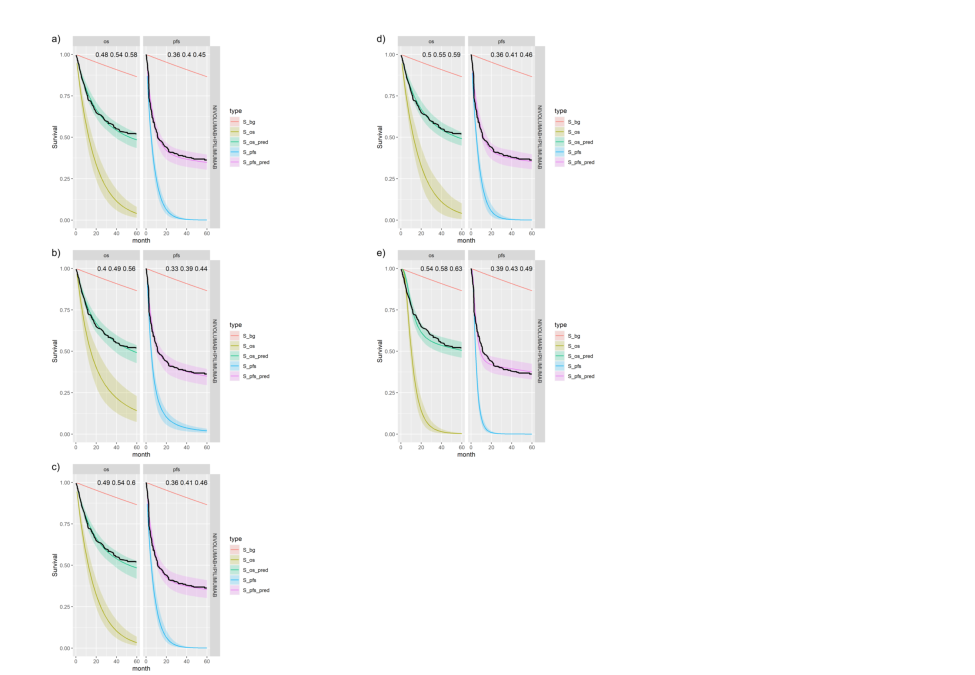
\includegraphics{how_to_use_files/figure-latex/unnamed-chunk-14-1.pdf}

\end{document}
